\section{Issues} \label{sec:issues}

\subsection{Zero Probabilities in Learned CPTs}
It was noticed that some of the conditional probability tables that Pomegranate learned from the data set (i.e., by solving the structure learning problem defined in Subsection \ref{subsec:learning-bn-structure}) presented entries with $0$ value.

The assignment of the extreme probabilities $1$ and $0$, while perfectly coherent in the frequentist approach, is not in line with the Bayesian one.
This is because of the different conception of probabilities between the two approaches, as discussed in Subsection \ref{subsec:probability-interpretations}.
A frequentist practitioner would happily assign probability zero to an event not present in the data set while a Bayesian would refrain in doing so, as having a zero or one prior belief makes every posterior, calculated using Bayes' Rule (Definition \ref{th:bayes-theorem}), also zero or one.
The necessity of avoiding the assignment of prior probability beliefs equal to $0$ or $1$, has been named \enquote{Cromwell's rule} by \citet{Jackman2009}.

A useful distinction to make that could help in deciding when to accept extreme probabilities or not, is between \textit{a priori} and \textit{a posteriori} propositions; the former are those whose truth value is not empirical but can, in general, be deduced based on logical necessity alone; the latter are those whose truth value is based on experience, for example any statement regarding the physical world.
An example of \textit{a priori} proposition could be a tautology, such as \enquote{every wife is married}; an example of \textit{a posteriori} proposition could be an assertion regarding the state of the world, for example \enquote{yesterday it rained}.
It would be an epistemological error to believe in the absolute truth or falsity of any proposition that is not necessary and thus one should refrain from assigning absolute belief or disbelief to their truth value.
This is because, apart from issues regarding the \textit{ontological determinism of Reality} and of the \textit{contingency of experience}, it is also against the intended use of statistics; statistical methods should only be applied in cases of uncertainty and not in those where a \textit{deterministic mechanism} is implied.
If a proposition's truth value can be known without resorting to the senses, then its value does not depend on the state of things in the sensible world.
Thus, we can assign absolute confidence in the truth value of a priori statements.

To solve the issue in the context of this work, a simple post-learning correction was applied; specifically a small positive constant was added to every zero-valued entry in the CPTs in Pomegranate's model.
The methodologically correct approach would have been to apply \textit{Laplace smoothing}, a standard technique used to \textit{smooth} categorical data.
The method would have entailed adding a \textit{pseudocount} $\alpha$ to every empirical probability estimated from the data set.
Given $x_i$ the count of occurrences of event $i$ in a set of $N$ events, the un-smoothed empirical probability is:
\begin{equation}
	p_i = \frac{x_{i}}{N} \,,
\end{equation}
while the smoothed one would be given by:
\begin{equation}
	p_i^*=\frac{x_{i}+\alpha}{N+\alpha d} \,,
\end{equation}
with $d$ the number of possible categories.

The value of $\alpha$ should be chosen to reflect any prior knowledge regarding the events; in the case there were none, a non-informative prior should be chosen, as stated by the \textit{principle of indifference} (in absence of any evidence one should distribute his beliefs uniformly).
The simplest possible non-informed approach is to increment every event's count in the data set by one, including the ones not appearing.
Thus the relative frequency between events will be maintained but there will be no event $i : x_i=0=p_i$.

Unfortunately implementing this approach, while recognisably the most methodologically sound way of proceeding, would have been very time-consuming and outside the main focus of this thesis.
The chosen strategy of adding a small positive constant $\epsilon$ to each empirical probability $p_i$, while not strictly correct, is extremely unlikely to change the learned CPTs.
This cannot be ruled out \textit{a priori} and would require \textit{sensitivity analysis} to be decided, but we are working with the prior belief that this is very unlikely to happen.

The developed algorithm, termed \enquote{epsilon smoothing}, is based on adding and subtracting \enquote{probability atoms} $\epsilon$ with the objective of removing zeros in the CPTs and maintaining the normalisation, so that the result will still be a valid probability distribution (based on Definition \ref{def:probability-measure}).
We work with probability atoms $\epsilon$ so as not to incur in numerical imprecisions in the implementation, as only additions and subtractions need to be used.
Every zero-valued element in a CPT column has a quantity $\epsilon \times \#!0$ added to it, with $\#!0$ the number of elements in the distribution that are not zero, and every non-zero entry has $\#0$, the number of zero elements, atoms subtracted from it.
The end result is obviously still a correctly normalised probability distribution because given a probability distribution $P$, with $n$ elements $p_i$ of which $\#0$ are zero, and the  distribution $P^*$ resulting from to the described procedure:
\begin{align}
	&\sum\limits_{i=0}^{n} p_i = 1 \\
	\wedge  \quad &1 - \{ \#0 \times [(n - \#0) \times \epsilon] \} + \{ (n - \#0) \times [\#0 \times \epsilon] \}  = 1 \\
	\implies \quad  &\sum\limits_{i=0}^{n} p^*_i = 1
\end{align}
The pseudocode is shown in Algorithm \ref{alg:epsilon-smoothing}.

\begin{algorithm}[htp!]
	\caption{Epsilon Smoothing algorithm pseudocode}
	\label{alg:epsilon-smoothing}
	\begin{algorithmic}[1]
		\State $\epsilon=$ smallest positive constant
		\For{$s$ in model CPTs}
			\For{$c$ in $s$'s columns} \Comment{distributions of values are organised column-wise}
				\State $num\_zeros$ = number of zero-valued entries in $c$
				\State $num\_non\_zeros$ = $|c|$ - $num\_zeros$
				\For{$v$ in $c$}
					\If{$v$ equal to $0$}
						\State $v += \epsilon \times num\_non\_zeros$
					\Else
						\State $v -= \epsilon \times num\_zeros$
					\EndIf
				\EndFor
			\EndFor
		\EndFor
	\end{algorithmic}
\end{algorithm}

If the procedure were applied to the CPT in Table \ref{tab:rec-cpd-issues}, it would yield the one shown in Table \ref{tab:rec-cpd-epsilon}.

\begin{table*}[htbp]
\centering
\caption{\enquote{recettori estrogeni} CPT}
\begin{tabularx}{0.5\textwidth}{ccXX}
\toprule
      & &  \multicolumn{2}{c}{\textbf{mut17q21}} \\
\cmidrule(lr){3-4}
 & & 0 & 1    \\ 
 \multirow{3}{*}{\textbf{rec. estr.}}  & 0 & $0.68 - \epsilon$ & 0.13  \\
 & 1 & $0.0 + 2\epsilon$ & 0.02    \\
 & 2 & $0.31 - \epsilon$ & 0.84 \\
\bottomrule
\end{tabularx}
\label{tab:rec-cpd-epsilon}
\end{table*}


\subsection{MPE Calculation} \label{subsec:results-mpe-calculation-issues}
The main issue encountered during the implementation of the system described in Section \ref{sec:implemented-tool}, was that of correctly calculating the MPE.
Initially, an attempt was made to write a custom function \texttt{export\_model\_to\_uai} to generate a UAI file (described in \ref{subsec:libraries}) directly from the Pomegranate Bayesian network model.
This UAI file was fed to DAOOPT to generate the MPE solution as recounted in Subsection \ref{subsec:algorithms} under the \enquote{MPE Algorithms Comparison} header.
When compared with the MPE solution generated directly using Pgmpy's \texttt{map\_query} function, it was seen that these disagreed in almost all cases.
This shouldn't have been the case as both were generated using exact methods: \textit{variable elimination} in Pgmpy's case and \textit{AND/OR branch-and-bound} for DAOOPT.

While investigating the cause for this divergence, an undocumented feature of Pgmpy was discovered: a \texttt{UAIWriter} class that should have converted the Pgmpy-based model (which was converted in turn from the Pomegranate-based model, as outlined in Subsection \ref{subsec:algorithms} at the \enquote{Pairwise Correlations} header) to the correct UAI file representing it.
When this alternative UAI file was used as input for DAOOPT, the resulting MPE not only diverged from that calculated based on \texttt{export\_model\_to\_uai}, as was to be expected, but also from that calculated directly with Pgmpy using \texttt{map\_query}, which was surprising.

The data flow for the MPE calculation is shown in Figure \ref{fig:mpe_conversion_process}; initially a Pomegranate-based BN is learned from the data set by using the built-in \texttt{from\_samples} method, then a custom \texttt{convert\_to\_pgmpy} function converts the Pomegranate-based model to a Pgmpy-based one.
The custom function \texttt{export\_to\_uai} and Pgmpy's built-in \texttt{UAIWriter} class are used to generate the \texttt{.uai} and \texttt{.uai.evid} files that are the input for DAOOPT to generate the MPE solutions.
The \texttt{map\_query} method that is part of Pgmpy's API is also used to generate an MPE assignment.

\begin{figure}[htbp]
\centerline{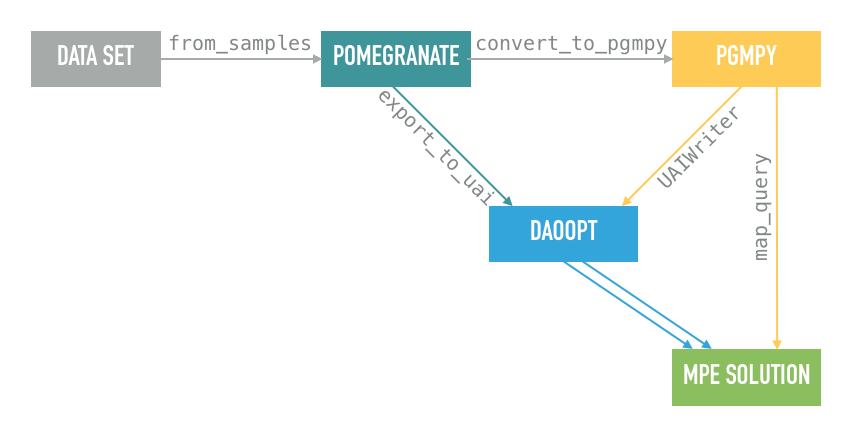
\includegraphics[width=\textwidth]{results/images/mpe_conversion_process}}
\caption{MPE calculation flow.}
\label{fig:mpe_conversion_process}
\end{figure}

The conversion from the Pomegranate-based to the Pgmpy-based model was thoroughly tested using conditional probability and independencies queries, so the issue is most likely to be found elsewhere.
As the DAOOPT MPE solution generated starting from the UAI differs from the one calculated directly with Pgmpy, there must be a bug either in Pgmpy's UAI exporter or in its inference method.
It is unclear if Pgmpy is still presenting issues in its inference methods\footnote{\url{https://github.com/pgmpy/pgmpy/issues/856}} but a series of tests on simple networks, where the MPE calculations were carried out manually, seemed to confirm that \texttt{map\_query} was returning the correct MPE solution.

For example, in the small BN whose structure is shown in Figure \ref{fig:issues-bn} and the CPDs of the nodes in Tables \ref{tab:mut-cpd-issues}, \ref{tab:eta-cpd-issues}, \ref{tab:rec-cpd-issues} and \ref{tab:diff-cpd-issues}, Pgmpy's \texttt{map\_query} and DAOOPT returned different solutions to the following MPE query:
\begin{align}
\begin{split}
	\text{MPE}( \text{\enquote{differenziazione}}=x, \text{\enquote{mut17q21}}=y, \text{\enquote{recettori estrogeni}}=z \\
	\mid \text{\enquote{eta arrotondata}}=0 )
\end{split} 
\end{align}
\texttt{map\_query} returned the assignment: 
\begin{align} \label{eq:pgmpy-assignment}
  (\text{\enquote{differenziazione}}=1, 
  \text{\enquote{mut17q21}}=1, 
  \text{\enquote{recettori estrogeni}}=2)
\end{align}
while DAOOPT on the UAI exported with Pgmpy's returned:
\begin{align} \label{eq:daoopt-assignment}
  (\text{\enquote{differenziazione}}=0, 
  \text{\enquote{mut17q21}}=1, 
  \text{\enquote{recettori estrogeni}}=2)
\end{align}

In such a small network it is easy to verify that the probability of Equation \ref{eq:pgmpy-assignment} is: $0.99 \times 0.84 \times 0.60 = 0.50$ and that it is the MPE solution.
The fact that the probability of Equation \ref{eq:daoopt-assignment} is $0.99 \times 0.84 \times 0.21 = 0.17$, makes it obviously incorrect.

\begin{figure}[htbp]
\centerline{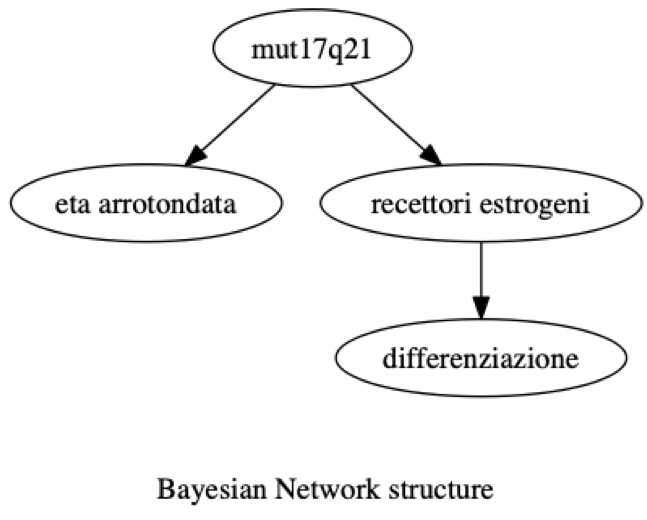
\includegraphics[width=0.5\textwidth]{results/images/issues-bn}}
\caption{Independencies query natural language output.}
\label{fig:issues-bn}
\end{figure}

\begin{table*}[htbp]
\centering
\caption{\enquote{mut17q21} distribution}
\begin{tabularx}{\textwidth/3}{ccX}
\toprule
 \multirow{2}{*}{\textbf{mut17q21}} & 0 & 0.01  \\
 & 1 & 0.99 \\
\bottomrule
\end{tabularx}
\label{tab:mut-cpd-issues}
\end{table*}

\begin{table*}[htbp]
\centering
\caption{\enquote{eta arrotondata} CPT}
\begin{tabularx}{0.5\textwidth}{ccXX}
\toprule
      & &  \multicolumn{2}{c}{\textbf{mut17q21}} \\
\cmidrule(lr){3-4}
 & & 0 & 1    \\ 
 \multirow{3}{*}{\textbf{eta arr.}}  & 0 & 0.42 & 0.04  \\
 & 1 & 0.42 & 0.17    \\
 & 2 & 0.15 & 0.78 \\
\bottomrule
\end{tabularx}
\label{tab:eta-cpd-issues}
\end{table*}

\begin{table*}[htbp]
\centering
\caption{\enquote{recettori estrogeni} CPT}
\begin{tabularx}{0.5\textwidth}{ccXX}
\toprule
      & &  \multicolumn{2}{c}{\textbf{mut17q21}} \\
\cmidrule(lr){3-4}
 & & 0 & 1    \\ 
 \multirow{3}{*}{\textbf{rec. estr.}}  & 0 & 0.68 & 0.13  \\
 & 1 & 0.0 & 0.02    \\
 & 2 & 0.31 & 0.84 \\
\bottomrule
\end{tabularx}
\label{tab:rec-cpd-issues}
\end{table*}

\begin{table*}[htbp]
\centering
\caption{\enquote{differenziazione} CPT}
\begin{tabularx}{0.5\textwidth}{ccXXX}
\toprule
      & &  \multicolumn{3}{c}{\textbf{recettori estr.}} \\
\cmidrule(lr){3-5}
 & & 0 & 1 & 2   \\ 
 \multirow{3}{*}{\textbf{diff.}}  & 0 & 0.012 & 0.16 & 0.21  \\
 & 1 & 0.18 & 0.43 & 0.60    \\
 & 2 & 0.80 & 0.40 & 0.18 \\
\bottomrule
\end{tabularx}
\label{tab:diff-cpd-issues}
\end{table*}

\subsection{Late Removal of Clinical Variables} \label{subsec:removal-clinical-variables}
As discussed in Section \ref{sec:data-set}, it was decided to drop certain variables from the initial data set.
Among these, \enquote{mut17q21}, \enquote{loss 17} and \enquote{FISHRatio} were initially included in the post-processed data set and became part of the Bayesian network.
Thus, in the initial phases of development and validation the network topology was the one shown in Figure \ref{fig:old-bn-plot}, which can be compared with the current one shown in Figure \ref{fig:sw_plot_result}.

\begin{figure}[htbp]
\centerline{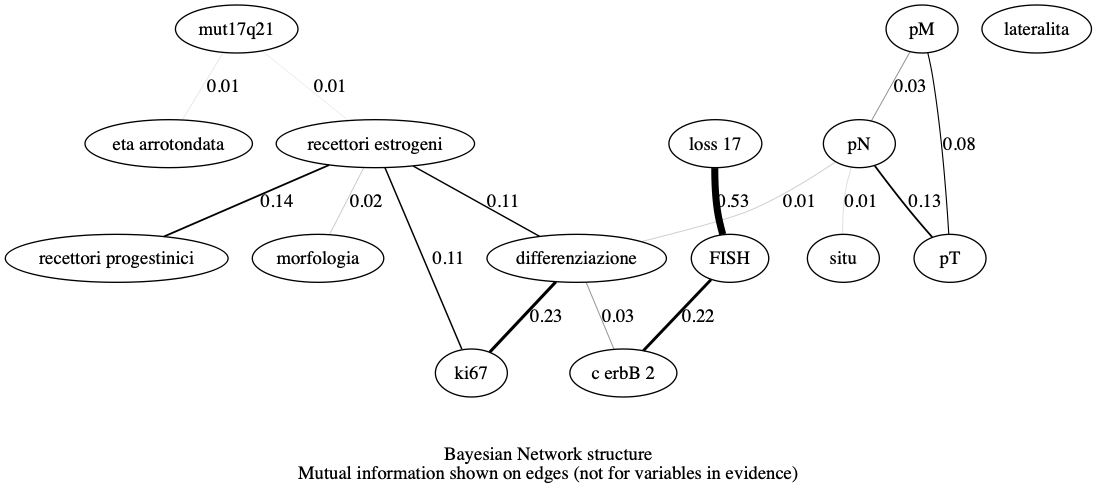
\includegraphics[width=\textwidth]{results/images/old-bn-plot}}
\caption{Bayesian network topology before the removal of \enquote{mut17q21}, \enquote{loss 17} and \enquote{FISH}.}
\label{fig:old-bn-plot}
\end{figure}

At a later phase a decision was made, in agreement with the ICP, to remove these three variables from the data set during the preprocessing phase; this was due to their being extremely skewed in their values, as can be seen by inspecting the \enquote{Distribution} column in Table \ref{tab:datasetdistribution}.

The reason for their skewness was briefly mentioned in Subsection \ref{subsec:motivation} and can be traced to the fact that these variables are all connected to the technique of \textit{fluorescence in situ hybridisation}.
This can be understood by analysing the \enquote{Clinical meaning} column in Table \ref{tab:datasetvariables} and knowing that FISH enables the analysis of specific DNA sequences on chromosomes and in particular of chromosome 17, because of its significance in breast cancer \citep{zhang2011important}.
FISH was a technique that was not available prior to 2010 and thus nearly 70\% of the patients in the data set had a value of \enquote{NCO} for \enquote{FISHRatio}, meaning this test had not been carried out on them.
Even worse, \enquote{mut17q21} presented more than 99\% \enquote{unknown} values and \enquote{loss 17} had 78\% of \enquote{FISH non fatta/FISH non valutabile}, meaning that the great majority of cases presented values with no real clinical meaning.

It can be seen in Figure \ref{fig:old-bn-plot} how strong the association between \enquote{loss 17} and \enquote{FISH} was - \textit{a posteriori}, a clear case of spurious correlation - and how feebly \enquote{mut17q21} was connected to the rest of the network.
Having these variables was introducing a very large amount of bias that confounded the resulting model.
An example of this effect was experienced in the early stages of validation; a previous series of validation questions had been prepared by the ICP and included queries in a form similar to:
\begin{quotation}
	In the general population, if \textit{[...]} is \textit{[...]}, then is it more/less probable that \textit{[...]} is \textit{[...]}?
\end{quotation}
and
\begin{quotation}
	In young patients, if \textit{[...]} is \textit{[...]}, then is it more/less probable that \textit{[...]} is \textit{[...]}?
\end{quotation}
Queries of these forms, when compared against each other, reliably returned identical answers, indicating that the age of the patient (\enquote{eta arrotondata} in the benchmark data set) had little or no influence of the values of other variables.
Inspection of Figure \ref{fig:sw_plot_result} will show how, after the removal of \enquote{mut17q21}, \enquote{loss 17} and \enquote{FISHRatio}, \enquote{eta arrotondata} actually becomes disconnected from the rest of the network.
The removal of the spurious \enquote{bridge} created by \enquote{mut17q21} now explicitly shows and confirms that patient age can have no influence on other variables' values, as had already been noticed before removal. 

The ICP confirmed that removing these three variables helped its users in better understanding the differences between a correlation in the variables representing the data set and a correlation in the actual clinical meaning behind the data.
That is, they felt that it reduced the \textit{confounding factors} thus allowing a better appreciation of the explainability methods used.